La figura \ref{fig:presupuesto_costes} muestra de forma detallada el presupuesto de costes con todos los costes del proyecto.  Los valores utilizados para la realización del presupuesto son los siguientes:
\begin{itemize}
	\item Las horas de trabajo totales serán las obtenidas en la ``\nameref{planificacion:inicial}''. En total 820h.
	\item El número de horas de trabajo diarias será de 8h con 20 jornadas de trabajo mensuales.
	\item El porcentaje del salario del desarrollador destinado a la seguridad social será del 35\%.
\end{itemize}


	\begin{figure}[h]
		\centering
		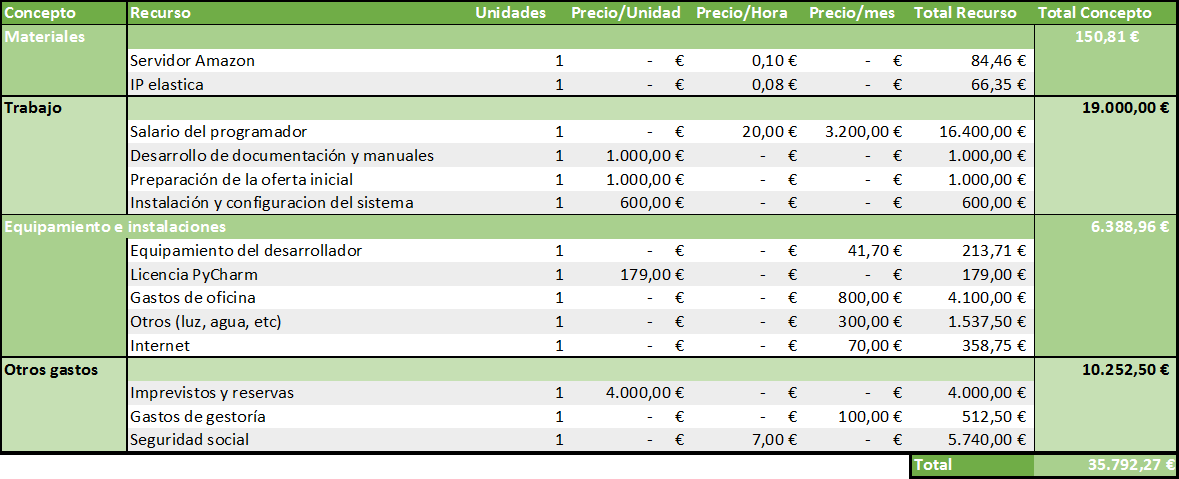
\includegraphics[width=\textwidth]{presupuesto/costes}
		\caption{Presupuesto de costes del proyecto}
		\label{fig:presupuesto_costes}
	\end{figure}

El presupuesto de costes está dividido en 4 categorías que se describirán a continuación

\subsection{Materiales}
	Los materiales se refieren al hardware y software con los que se quedará el cliente después de finalizar el desarrollo, pero que tendrán un coste durante el mismo.
	\begin{itemize}
		\item El \textbf{servidor} utilizado durante el desarrollo será un servidor \textit{Amazon EC2 m3.large}. El coste de éste servidor será de 0,14 \$ por cada hora de funcionamiento (sin IVA)\footnote{La información detallada de los precios de Amazon EC2 puede consultarse en \url{http://aws.amazon.com/es/ec2/pricing/}}.  Éste servidor correrá a cargo del equipo de desarrollo durante el proyecto, una vez finalizado el proyecto correrá a cargo del cliente.
		\item Una dirección \textbf{elastic IP} permite asignar una misma dirección IP a diferentes instancias y conservarla sin que se modifique al apagar o encender la máquina.  El coste de éste servicio es de 0,11 \$ por hora (sin IVA).
	\end{itemize}

\subsection{Trabajo personal}
	El trabajo personal se refiere al trabajo realizado por los desarrolladores del proyecto.
	
	El salario del desarrollador será de \EUR{20}  por cada hora de trabajo, lo que equivale a \EUR{3200}  mensuales trabajando 8 horas diarias durante 20 días al mes.  En total resulta en \EUR{16400} para todo el proyecto.
	
	También se incluye el coste del desarrollo de la documentación y los manuales que se entregarán al cliente, así como la instalación y configuración del sistema y la preparación de la oferta inicial, conjuntamente tienen un coste de \EUR{2600}.

\subsection{Equipamiento e instalaciones}
	Se incluyen aquí todos los costes relativos al equipamiento utilizado por los desarrolladores así como las instalaciones en las que se efectuará el trabajo.
	
	El lugar de trabajo será una oficina especialmente dedicada, con un coste de \EUR{800} cada mes, lo que produce un coste de \EUR{4100} para el proyecto.  Al coste de la oficina se añadirán los gastos de agua, luz e Internet, conjuntamente tienen un coste de \EUR{1896,25} en el proyecto.\\
	Además también se incluirá en ésta partida el gasto necesario para amortizar el equipamiento del desarrollador.  El equipamiento ha tenido un coste inicial de \EUR{1500} y se espera amortizar en 3 años (36 meses).  El coste de amortización de éste equipamiento es de \EUR{41,70} mensuales, lo que produce un coste de \EUR{213,71} a lo largo del proyecto.
	
	Por último, se incluye también el precio del entorno de desarrollo integrado utilizado por el desarrollador, éste tiene un coste de \EUR{179}\footnote{La información detallada sobre el precio de éste componente puede consultarse en \url{http://www.jetbrains.com/pycharm/buy/}}.
	
\subsection{Otros gastos}
	En ésta partida se incluyen el resto de gastos que afectan al proyecto y no forman parte de las partidas anteriores.  Se incluye aquí un fondo para posibles imprevistos que surjan a lo largo del desarrollo, éste fondo está valorado en \EUR{4000}.
	
	También se incluyen los gastos de gestoría con un coste de \EUR{100} mensuales, lo que resulta en \EUR{512,50} para el proyecto completo.  Los costes de la seguridad social del desarrollador se calculan tomando el 35\% de su salario, lo que resulta en \EUR{7} a la hora y \EUR{5740} a lo largo del proyecto.
	
\subsection{Total}
	Tras sumar los costes de todas las partidas se obtiene un coste total del proyecto de \EUR{35792,27}.  Puesto que éste es el presupuesto de costes, no se incluirán los impuestos.  Los impuestos serán incluidos en el presupuesto del cliente tras aplicar el beneficio deseado.